\documentclass[a4paper,12pt]{article}
%%% Default imports
\usepackage{listings} % Code listings
\usepackage{graphicx} % Images
\usepackage{booktabs} % Better tables
\usepackage{makecell}
\usepackage{enumitem} % Lists
\usepackage{dsfont}
\usepackage{geometry} % Page geometry
\usepackage[utf8]{inputenc} % Encoding
\usepackage[T2A]{fontenc} % Font
\usepackage[english, russian]{babel} % Multi-language support
\usepackage{titling} % Better titles
\usepackage{textcomp} % Old-style numbers? Check difference
\usepackage{mathtext} % Russian text in math expressions? Check difference
\usepackage{amsmath, amsfonts, amssymb, amsthm, mathtools} % Mathematics
\usepackage{bm} % Bold math symbols
\usepackage{icomma} % Better comma in numbers within math mode
\usepackage{xifthen} % Better if-expressions
\usepackage{transparent} % Transparent colors
\usepackage{caption}    % }
\usepackage{subcaption} % } Captioning figures
\usepackage[table,xcdraw]{xcolor} % Colors
\usepackage{textpos} % Absolute positioning
\usepackage{upgreek} % Cool greek letters

\usepackage{fancyvrb}
\usepackage{fvextra}
\usepackage{chngcntr}

%%% Page geometry
\setlength\parindent{0pt} % No indentation between paragraphs
\setlist{noitemsep} % No spacing between list items

\usepackage{float}
\usepackage{multirow}

\geometry{
    paper=a4paper,
    top=2.5cm,
    bottom=3cm,
    left=2.5cm,
    right=2.5cm,
    headheight=0.75cm,
    footskip=1.5cm,
    headsep=0.75cm,
}

%%% Numeration
\newcommand{\RNumb}[1]{\uppercase\expandafter{\romannumeral #1\relax}}
\newcommand{\thesec}{\arabic{section}}
\renewcommand\thesection{\arabic{section}}
\renewcommand\thesubsection{\thesection.\arabic{subsection}}
\renewcommand\thesubsubsection{\RNumb{\arabic{subsubsection}}}
\renewcommand{\sectionmark}[1]{\markright{\thesection\ #1}}
\renewcommand{\bf}{\textbf}
\renewcommand{\it}{\textit}
\def\hash{\texttt{\#}}
\def\cpp{\C\texttt{++}}

\counterwithin{figure}{section}
\counterwithin{table}{section}
\renewenvironment{titlepage}{\thispagestyle{empty}} % Include titlepage into page numeration

%%% Headers and footers
\usepackage{setspace}
\usepackage{fancyhdr}
\usepackage{lastpage}


%%% Graphics
% Custom colors
\definecolor{myblue}{RGB}{72, 184, 178}
\definecolor{myblue1}{RGB}{0, 109, 167}
\definecolor{commentgreen}{RGB}{2,112,10}
\definecolor{mauve}{rgb}{0.58,0,0.82}
\definecolor{amethyst}{RGB}{153, 102, 203}

\usepackage{pgfplots} % Plots
\usepackage{tikz}
\usetikzlibrary{3d,perspective,decorations.text}
\usetikzlibrary{animations}
\usetikzlibrary{positioning}
\usetikzlibrary{matrix}
\usepackage{tikz-cd}
\usetikzlibrary{cd}
\usetikzlibrary{karnaugh}
\pgfplotsset{width=6cm,compat=newest}
\usepackage{color}

\usepackage[framemethod=TikZ]{mdframed}
\newcommand{\definebox}[2]{\newcounter{#1}\newenvironment{#1}[1][]{\stepcounter{#1}\mdfsetup{frametitle={\tikz[baseline=(current bounding box.east),outer sep=0pt]\node[anchor=east,rectangle,fill=white]{\strut \MakeUppercase#1~\csname the#1\endcsname\ifstrempty{##1}{}{:~##1}};}}\mdfsetup{innertopmargin=1pt,linecolor=#2,linewidth=3pt,topline=true,frametitleaboveskip=\dimexpr-\ht\strutbox\relax,}\begin{mdframed}[]\relax}{\end{mdframed}}}
\definebox{definition}{black!90}
\definebox{theorem}{myblue1!90}
\definebox{demonstration}{amethyst!90}

\newcounter{Theorem}
\def\themytheorem{\thesection.\arabic{Theorem}}
\usepackage[most]{tcolorbox}
\tcbuselibrary{theorems}
\newtcbtheorem{Theorem}{Theorem}
{colframe=myblue!90,coltitle=black,colback=white,fonttitle=\bfseries}{Th}

%%% Code listings
\usepackage{matlab-prettifier}

\lstdefinestyle{cpp} {
    language=C++,
    frame=tb,
    tabsize=4,
    showstringspaces=false,
    numbers=left,
    captionpos=b,
    columns=flexible,
    upquote=true,
    commentstyle=\color{commentgreen},
    keywordstyle=\color{blue},
    stringstyle=\color{commentgreen},
    basicstyle=\small\ttfamily,
    emph={int,char,double,float,unsigned,void,bool,size\_t},
    emphstyle={\color{blue}},
    escapechar=\&,
    classoffset=1,
    otherkeywords={>,<,.,;,-,!,=,~},
    morekeywords={>,<,.,;,-,!,=,~},
    keywordstyle=\color{black},
    classoffset=0,
}
\lstdefinestyle{def} {
    frame=tb,
    tabsize=4,
    showstringspaces=false,
    numbers=left,
    captionpos=b,
    columns=flexible,
    upquote=true,
    commentstyle=\color{black},
    keywordstyle=\color{black},
    stringstyle=\color{black},
    basicstyle=\small\ttfamily,
    emph={int,char,double,float,unsigned,void,bool,size\_t},
    emphstyle={\color{black}},
    escapechar=\&,
    classoffset=1,
    otherkeywords={>,<,.,;,-,!,=,~},
    morekeywords={>,<,.,;,-,!,=,~},
    keywordstyle=\color{black},
    classoffset=0,
}
\lstdefinelanguage[RISC-V]{Assembler}
{
    alsoletter={.}, % allow dots in keywords
    alsodigit={0x}, % hex numbers are numbers too!
    morekeywords=[1]{ % instructions
    lb, lh, lw, lbu, lhu,
    sb, sh, sw,
    sll, slli, srl, srli, sra, srai,
    add, addi, sub, lui, auipc,
    xor, xori, or, ori, and, andi,
    slt, slti, sltu, sltiu,
    beq, bne, blt, bge, bltu, bgeu,
    j, jr, jal, jalr, ret,
    scall, break, nop
},
    morekeywords=[2]{ % sections of our code and other directives
    .align, .ascii, .asciiz, .byte, .data, .double, .extern,
    .float, .globl, .half, .kdata, .ktext, .set, .space, .text, .word
},
    morekeywords=[3]{ % registers
    zero, ra, sp, gp, tp, s0, fp,
    t0, t1, t2, t3, t4, t5, t6,
    s1, s2, s3, s4, s5, s6, s7, s8, s9, s10, s11,
    a0, a1, a2, a3, a4, a5, a6, a7,
    ft0, ft1, ft2, ft3, ft4, ft5, ft6, ft7,
    fs0, fs1, fs2, fs3, fs4, fs5, fs6, fs7, fs8, fs9, fs10, fs11,
    fa0, fa1, fa2, fa3, fa4, fa5, fa6, fa7
},
    morecomment=[l]{;},   % mark ; as line comment start
    morecomment=[l]{\#},  % as well as # (even though it is unconventional)
    morestring=[b]",      % mark " as string start/end
    morestring=[b]'       % also mark ' as string start/end
}
\lstdefinestyle{riscv} {
    basicstyle=\small\ttfamily,                    % very small code
    breaklines=true,                              % break long lines
    commentstyle=\itshape\color{green!50!black},  % comments are green
    keywordstyle=[1]\color{blue!80!black},        % instructions are blue
    keywordstyle=[2]\color{orange!80!black},      % sections/other directives are orange
    keywordstyle=[3]\color{red!50!black},         % registers are red
    stringstyle=\color{mauve},                    % strings are from the telekom
    identifierstyle=\color{teal},                 % user declared addresses are teal
    frame=l,                                      % black line on the left side of code
    captionpos=b,
    language=[RISC-V]Assembler,                   % all code is RISC-V
    tabsize=4,                                    % indent tabs with 4 spaces
    showstringspaces=false                        % do not replace spaces with weird underlines
}

%%% Other
\usepackage[normalem]{ulem} % }
\useunder{\uline}{\ul}{}    % } Underline text
\usepackage[colorlinks,urlcolor=blue,filecolor=blue,citecolor=blue,linkcolor = blue,unicode=true]{hyperref}
\usepackage{titlesec}
\titlelabel{\thetitle.\quad}
\usepackage{secdot}
\sectiondot{subsection}
\usepackage{kvmap} % Karnaugh-maps for logic functions
\usepackage{}
\newcommand{\projectname}[3]{
    \begin{center}
        \Large
        \textbf{#1}\\[10pt]
        \textbf{#2}\\[10pt]
        \normalsize
        #3
        \rule{\linewidth}{0.4pt}
    \end{center}
}

\newcommand{\hfconfiguration}[3]{
    \pagestyle{fancy}
    \fancyhead[LE,RO]{}
    \fancyhead[LO,RE]{#1}
    \renewcommand{\footrulewidth}{0.4pt}
    \fancyfoot[C]{\thepage/\pageref*{LastPage}}
    \fancyfoot[LO,RE]{#2}
    \fancyfoot[LE,RO]{#3}
}

\newcommand{\filename}[2]{
    \pagebreak
    \titleformat{\section}
    [display]
    {\bfseries\Large}
    {}
    {0ex}
    {
        \vspace{-4.5ex}
        % \rule{\textwidth}{1pt}
        #1 \centering
    % \vspace{1ex}
    }
    [
        \normalfont\large
        #2
        \rule{\textwidth}{0.4pt}
        \normalsize
    ]
}

\newcommand{\project}[6]{
    \projectname{#1}{#2}{#3}
    \pagestyle{empty}
    \tableofcontents
    \newpage
    \hfconfiguration{#4}{#5}{#6}
}
%%% Final touch
\usepackage{subfiles}

\graphicspath{{polytech/etc/os/subfiles/images/}}

\begin{document}
    \begin{titlepage}
    \begin{center}
        \large Санкт-Петербургский политехнический университет Петра Великого\\
        \large Институт компьютерных наук и технологий \\
        \large Кафедра компьютерных систем и программных технологий\\[6cm]


        \huge Р Е Ф Е Р А Т\\[0.5cm]
        \large по дисциплине <<Основы операционных систем>>\\[0.1cm]
        \large\textbf{Файловая система FAT}\\[5cm]
    \end{center}


    \begin{flushright}
        \begin{minipage}{0.25\textwidth}
            \begin{flushleft}

                \large\textbf{Работу выполнил:}\\
                \large Калашников О.Ю.\\
                \large {Группа:} 35300901/10005\\

                \large \textbf{Преподаватель:}\\
                \large Малышев И.А.

            \end{flushleft}
        \end{minipage}
    \end{flushright}

    \vfill

    \begin{center}
        \large Санкт-Петербург\\
        \large \the\year
    \end{center}
\end{titlepage}

\vfill
\newpage
    
    \hfconfiguration{Файловая система FAT}{}{} 
    
    \tableofcontents
    
    \section{Вступление}

    Файловая система FAT изначально была разработана в 1970-х годах Марком МакДональдом и Биллом Гейтсом для использования на дискетах, и стала стандартом в MS-DOS и ранних версиях Windows. Несмотря на свой довольно большой возраст, FAT до сих пор используется на флэшках и некоторых других твердотельных накопителях. За всю свою историю она подверглась множеству изменений, однако сохранила свои ключевые идеи.

    \section{Сравнение с NTFS}

    Стандартом в Windows сейчас является современная файловая система NTFS, которая по многим характеристикам заметно обгоняет наиболее популярные версии FAT. Разница в характеристиках представлена в таблице~\ref{tab:ntfs}
    
    \begin{table}[H]
        \centering
        \begin{tabular}{|c|c|c|c|c|}
        \hline
                                                                              & NTFS                                                                      & FAT32                                                                    & FAT16                                                                    & FAT12                                                                    \\ \hline
        \begin{tabular}[c]{@{}c@{}}Максимальный\\ размер раздела\end{tabular} & 2ТБ                                                                       & 32ГБ                                                                     & 4ГБ                                                                      & 16Мб                                                                     \\ \hline
        \begin{tabular}[c]{@{}c@{}}Максимальный\\ размер файла\end{tabular}   & 16ТБ                                                                      & 4ГБ                                                                      & 2ГБ                                                                      & $<$16Мб                                                                  \\ \hline
        Размер блока                                                          & 4КБ                                                                       & $4 - 32$ КБ                                                              & $2 - 64$ КБ                                                              & $0.5 - 4$ КБ                                                             \\ \hline
        Отказоустойчивость                                                    & Да                                                                        & Нет                                                                      & Нет                                                                      & Нет                                                                      \\ \hline
        Сжатие                                                                & Да                                                                        & Нет                                                                      & Нет                                                                      & Нет                                                                      \\ \hline
        Совместимость                                                         & \begin{tabular}[c]{@{}c@{}}Windows\\ 10/8/7/XP/\\ Vista/2000\end{tabular} & \begin{tabular}[c]{@{}c@{}}Windows\\ ME/2000/\\ XP/7/8.1/10\end{tabular} & \begin{tabular}[c]{@{}c@{}}Windows\\ ME/2000/\\ XP/7/8.1/10\end{tabular} & \begin{tabular}[c]{@{}c@{}}Windows\\ ME/2000/\\ XP/7/8.1/10\end{tabular} \\ \hline
        \end{tabular}
        \caption{Сравнение FAT и NTFS}
        \label{tab:ntfs}
    \end{table}
    
    \section{Устройство файловой системы}

    Первоначально следует отметить, что система FAT обладает высокой надежностью и эффективностью в хранении данных благодаря своей основной идее -- представлению каждого файла в виде списка связанных блоков. Эта концепция позволяет оптимально распределить информацию в файловой системе, обеспечивая быстрый доступ к данным, а также возможность быстрого обнаружения и устранения ошибок при их возникновении.

    В связи с этим, важной ролью в системе FAT играет таблица размещения файлов, которая содержит информацию о последовательности соединенных блоков. Таким образом, каждый файл имеет свой уникальный адрес, который помогает системе быстро находить его и обеспечивать управление им.
    \begin{figure}[H]
        \centering
        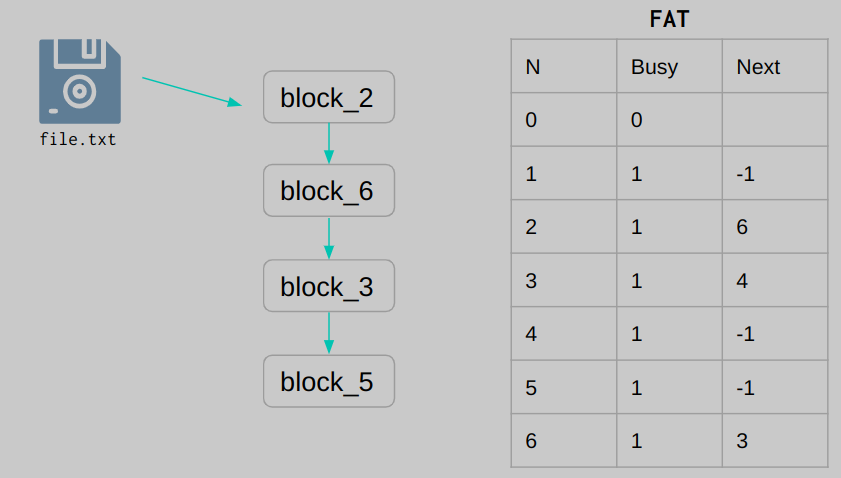
\includegraphics[width=0.8\linewidth]{img2}
        \caption{Пример работы таблицы размещения}
    \end{figure}
    В целях расширения функциональности системы разработчики добавили в нее таблицу каталогов, которая содержит информацию о том, какой блок в файле является первым. Эта таблица выступает важной связующей позицией между таблицей размещения файлов и фактическим расположением данных на диске.
    \begin{figure}[H]
        \centering
        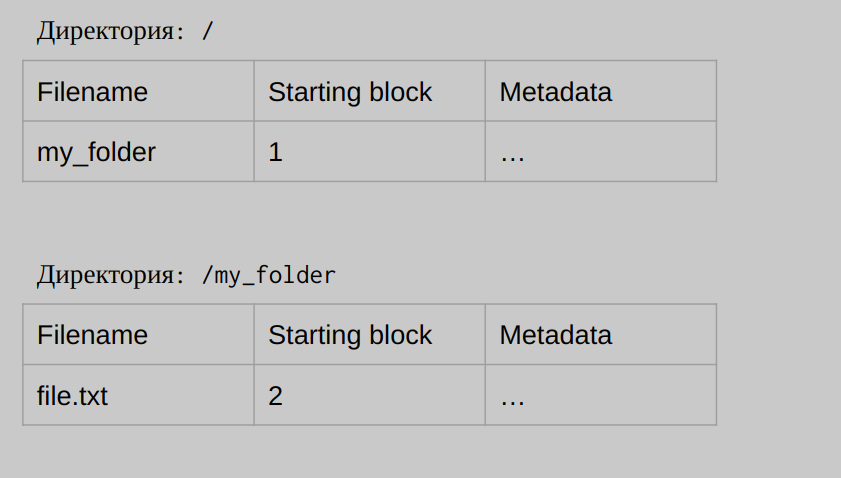
\includegraphics[width=0.8\linewidth]{img3}
        \caption{Пример работы таблицы каталогов}
    \end{figure}
    Однако при использовании системы FAT возникает некоторое количество вопросов, которые требуют дополнительных разъяснений. К примеру, как система определяет адрес root-директории? В данном случае стоит отметить, что адрес root-директории является зарезервированным и всегда известен системе. Это позволяет обеспечить корректную работу всей файловой системы, гарантированный доступ к данным и защиту от ошибок.
    
    Следовательно, использование системы FAT - это надежный и эффективный способ хранения информации, который обеспечивает быстрый доступ к данным, а также возможность быстрого обнаружения и устранения ошибок. Однако для полного понимания ее работы стоит изучить особенности ее устройства и принципов функционирования.

    \section{Практическая часть}
    
    Устройство файловой системы можно просмотреть на живом примере с помощью специализированных hex-редакторов.
    
    \begin{figure}[H]
        \centering
        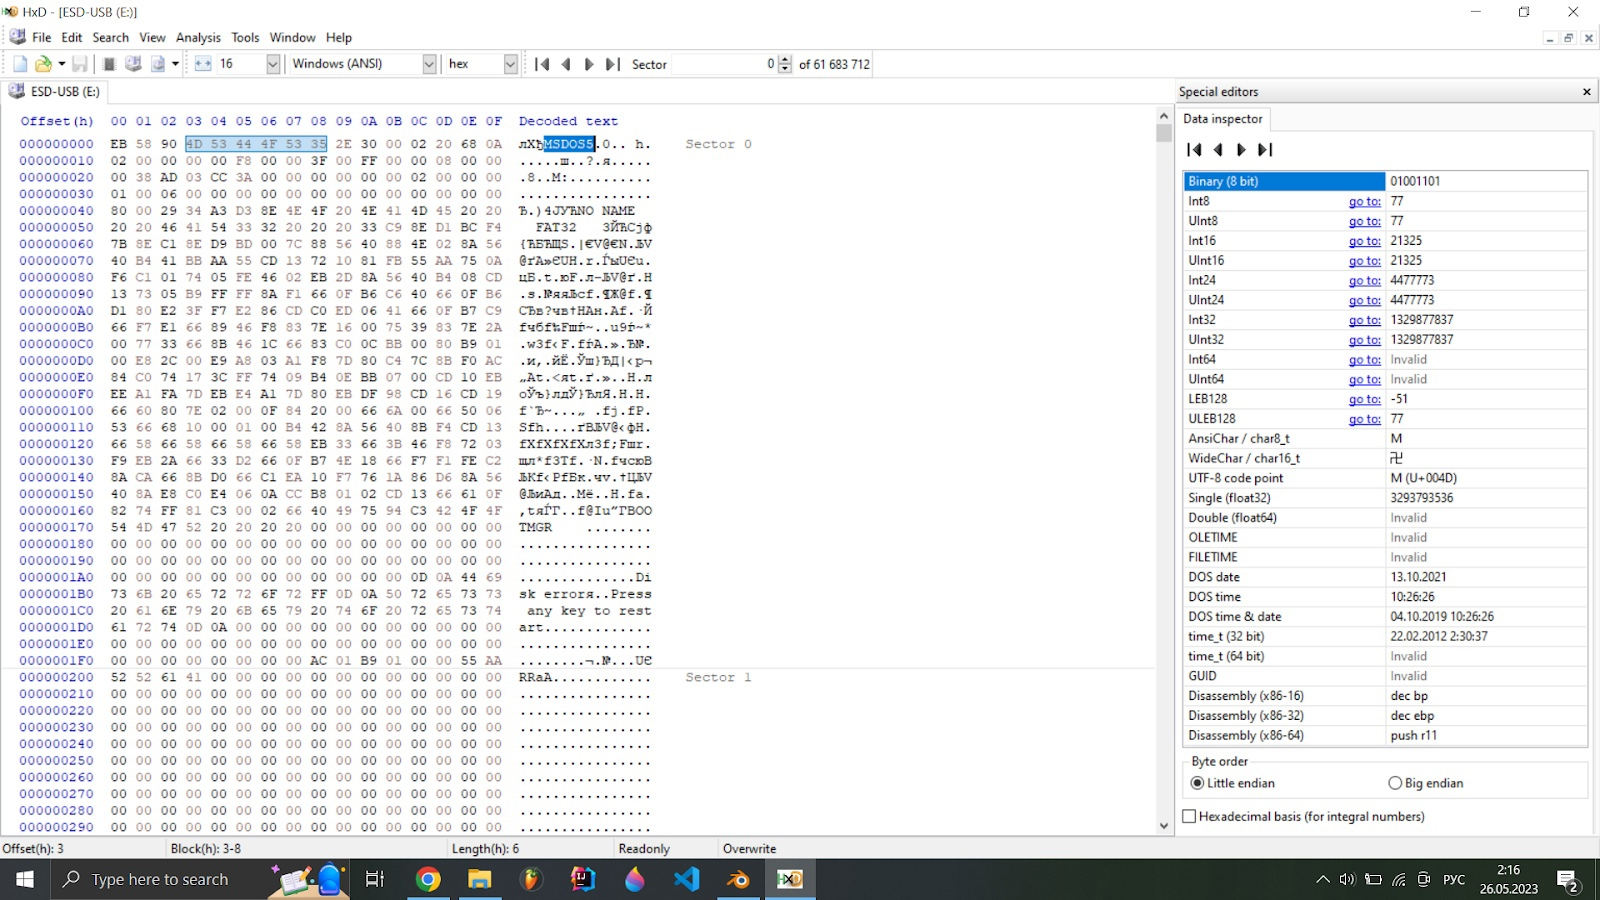
\includegraphics[width=\linewidth]{img1}
    \end{figure}

    С помощью ASCII-дешифратора справа от таблицы байтов можно сразу увидеть знакомые слова. В самой первой строчке присутствует запись «MSDOS5.0», которая обозначает операционную систему, на которой проводилось форматирование файловой системы. В целях сохранения обратной совместимости, обычно в этом поле указываются более старые системы, как, например, в данном случае, несмотря на то, что последнее форматирование проводилось на Windows 10. На строке $50$ видно обозначение файловой системы — FAT32.
    
    В байтах $0B_{16}$ и $0C_{16}$ записан размер сектора системы в байтах. В данном случае — $200_{16}$ = $512_{10}$. В байтах $0E_{16}$ и $0F_{16}$ содержится информация о количестве секторов, выделенных под резервную область файловой системы — $0A68_{16}$ = $2664_{10}$. С помощью этой информации можно узнать местонахождение самой файловой таблица, которая будет находится в секторе под номером $A68_{16}$. Прежде чем перейти к самой таблице, стоит обратить внимание ещё на некоторые значения: в байтах $32$ и $33$ хранится информация о местонахождении резервной копии метаданных — $0006$.
    
    \begin{figure}[H]
        \centering
        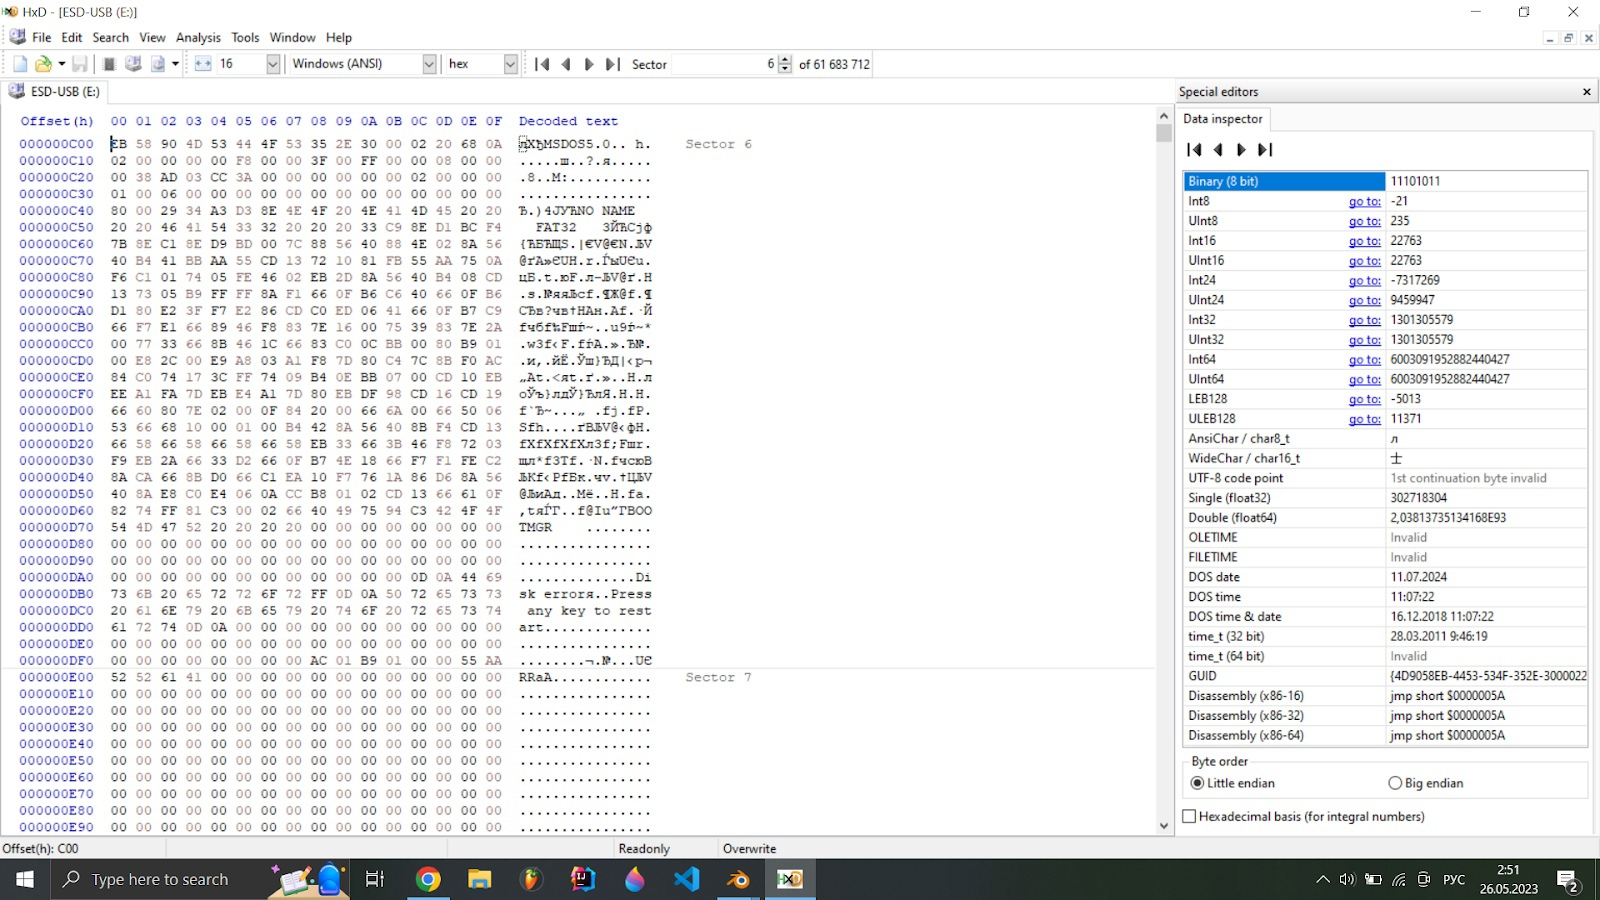
\includegraphics[width=\linewidth]{img0}
    \end{figure}
    
    Перейдя в сектор с номером $6$ можно действительно увидеть копию той информации, которая только что рассматривалась.
    
    \section{Список использованных источников}

    \begin{itemize}
        \item \url{https://www.udacity.com/course/gt-refresher-advanced-os--ud098}
        \item \url{https://shorturl.at/hnFWZ}
        \item \url{https://www.youtube.com/watch?v=FQ_xeY0eCpA&ab_channel=AlekOS}
    \end{itemize}

\end{document}